\documentclass[11pt]{article}

%	packages
\usepackage{tikz}
\usepackage{authblk}
\usepackage{amsmath}
\usepackage{amssymb} 
\usepackage{caption}
\usepackage{graphicx}
\usepackage[hypertexnames=false,colorlinks=true,linkcolor=blue,citecolor=blue]{hyperref}
\usepackage[numbers,comma,square,sort&compress]{natbib}
\usepackage[a4paper,text={6.5in,10in},centering]{geometry}
\usepackage{subcaption}
%	code syntax higlighting
\usepackage{listings}
\usepackage{color}
\usepackage{textcomp}
\definecolor{listinggray}{gray}{0.9}
\definecolor{lbcolor}{rgb}{0.9,0.9,0.9}
% C++ = [Visual]C++ ; matlab = matlab
\lstset{
	backgroundcolor=\color{lbcolor},
	tabsize=4,
	rulecolor=,
	language=java,
	keywordstyle=\bfseries\ttfamily\color[rgb]{0,0,1},
	identifierstyle=\ttfamily,
	commentstyle=\color[rgb]{0.133,0.545,0.133},
	stringstyle=\ttfamily\color[rgb]{0.627,0.126,0.941},
	showstringspaces=false,
	basicstyle=\small,
	%numberstyle=\footnotesize,
	%numbers=left,
	stepnumber=1,
	numbersep=10pt,
	tabsize=2,
	breaklines=true,
	prebreak = \raisebox{0ex}[0ex][0ex]{\ensuremath{\hookleftarrow}},
	breakatwhitespace=false,
	aboveskip={1.5\baselineskip},
  columns=fixed,
  upquote=true,
  extendedchars=true,
 frame=single,
% backgroundcolor=\color{lbcolor},
}


%	figures
\graphicspath{{eps/}{pdf/}{../figs//}}
%\setcaptionmargin{0.25in}
\def\captionfont{\itshape\small}
\def\captionlabelfont{\upshape\small}

%	counters
\makeatletter\@addtoreset{equation}{section}\makeatother
\renewcommand{\theequation}{\arabic{section}.\arabic{equation}}


%%%%%%%%%%%%%%%%%%%%%%%%%%%%%%%%%%%%%%%%%%%%%%%%%%%%%%%%%%%%%%%%%%%%%%%%%%%%

\begin{document}

\title{Equation-free analysis of agent-based models:\\Equation-free methods and implementation}

%\author[1]{Spencer A. Thomas}
\author{Spencer A. Thomas}
\author{David J.B. Lloyd}
\author{Anne C. Skeldon}
%\affil[1]{\small Department of Mathematics, Evolution and Resilience of Industrial Ecosystems (ERIE), University of Surrey, Guildford, GU2 7XH, UK}
\affil{\small Department of Mathematics, Evolution and Resilience of Industrial Ecosystems (ERIE), University of Surrey, Guildford, GU2 7XH, UK}
\date{\today}
\maketitle


%%%%%%%%%%%%%%%%%%%%%%%%%%%%%%%%%%%%%%%%%%%%%
% stochastic double well
%%%%%%%%%%%%%%%%%%%%%%%%%%%%%%%%%%%%%%%%%%%%%

\section{Numerical continuation}
\label{sec:NC}

In a numerical continuation approach, the focus is on fixed points 
(or periodic cycles). Rather than time evolving $x_{n+1} =f(x_n,\lambda)$ to find fixed points, solutions for $\tilde x$ such that
$ f(\tilde x, \lambda)-\tilde x = 0$ are sought. Having found a solution for one particular set of parameter values, 
the solution is `followed' by stepping in $\lambda$ and resolving
$ f(\tilde x, \lambda)-\tilde x = 0.$ The prediction method enables continuation along solution branches (Fig.~\ref{fig:NC}).
This is faster than finding fixed points using simulations and has the
advantage that both stable and unstable solutions can be found. These techniques are 
well-established in their value in understanding deterministic systems \cite{Allgower1990}. The also enable bifurcation and stability analysis of the system uncovering its behaviour under parameter variation. Although well studied for deterministic (no noise) systems, the application of this to stochastic (noisy) systems is extremely limited. Moreover this method requires the system to have an analytical form for the macroscopic state, i.e. an equation describing the systems behaviour. 

	\begin{figure}[h]
		\centering
		\includegraphics[width=0.9\linewidth, trim=6cm 19.5cm 6cm 4.5cm, clip=true]{PredictorCorrector}
		\caption{Pseudo-arclength predictor-corrector method (left) enabling continuation of both stable (solid) and unstable (dashed) solution branches (right). Based on known solutions (black) predictions can be made (white) for solutions under parameter perturbation. \label{fig:NC}}
	\end{figure}

\section{Equation-free Methods} 
\label{sec:EF}
Equation-free methods \cite{Theodoropoulos2000, Kevrekidis2003} enable numerical continuation of a system by replacing the macroscopic dynamical equation, $x_{n+1} =f(x_n,\lambda)$, with an ensemble of simulations at the microscopic level. Using an appropriate microscopic state, initialised from the macroscopic state (lifting), the macroscopic behaviour of the model can be estimated (restricting) from an ensemble of microscopic simulations ($N$ realisations) over a small time window $\tau$ (time-horizon). $N$ independent microscopic states ($x$) are initialised from the macroscopic state ($X$) at time $t=0$. After a simulating each microscopic state (i.e. time evolution) from $t=0$ to $t=\tau$, the $X(t=\tau)$ state is estimated from the distribution of microscopic final state, i.e. $g(x)$ at $x(t=\tau)$. That is, for a stochastic system, after the simulation (time evolution) the ensemble of renationalisations will be in different states, yielding a distribution, $g(x)$. We can estimate the macroscopic state, $X(t=\tau)$, from this distribution by taking some properties such as mean, variance, etc. An overview of this generic process is given in Fig.~\ref{fig:EF}. This enables the macroscopic analysis of a system, i.e. using numerical continuation, without the need for an explicit form. That is it does not require an equation of the system, such as a partial differential equation, to describe its behaviour, thus the term equation-free. Additionally this provides a platform for continuation of stochastic systems.

\begin{figure}[h]
	\centering
	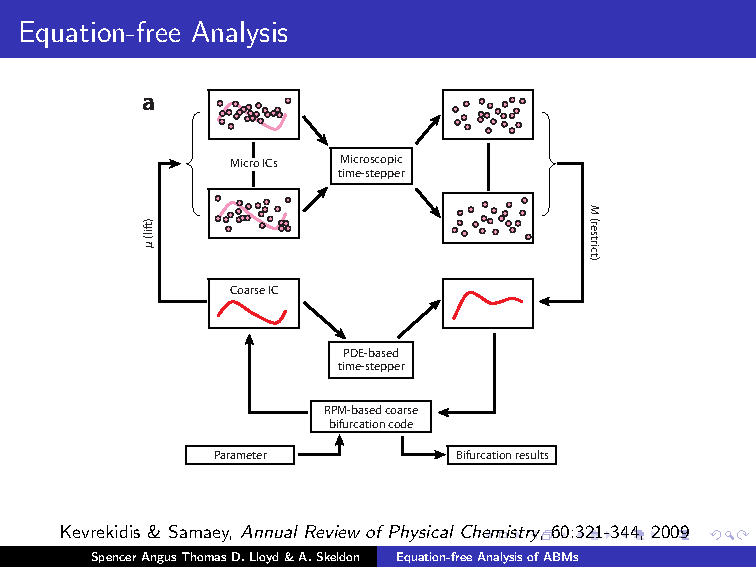
\includegraphics[width=\textwidth, trim= 1cm 1cm 1cm 1cm, clip=true]{EquationFreeOriginal}
	\caption{Equation-free method for macroscopic analysis figure from \cite{Kevrekidis2009}. IC-initial conditions, RPM-recursive predictor method and PDE-partial differential equation. \label{fig:EF}}
\end{figure}



\section{Implementation for agent-based models}
\label{sec:IMP}
In this instance we are interested in the analysis of agent-based models using the equation-free method described in Section~\ref{sec:EF}. Specifically, we use this process to perform numerical continuation of agent-based models as described in Section\ref{fig:NC}, which may be stochastic and rarely have an analytical form. We require our implemented algorithm to be generic, i.e. use-able for any agent-based model, and robust, i.e. is not sensitive to noise, parameters or the models themselves. 

Here we focus on NetLogo based agent-based models as it is commonly used in the research community, is compatible with all major operating system, and has the ability to interface with other languages enabling the construction of an equation-free `wrapper' to the models. In our code the Lifting step corresponds to the {\tt setup} procedure, the ensemble of realisations correspond to $N$ separate simulations run independently, the simulation (or time evolution) is the {\tt go} procedure. After the simulation of the realisations we take the mean of $g(x)$ as an estimator of $X(t=\tau)$. Our implementation of the equation-free process for agent-based models is illustrated in Fig.~\ref{fig:equationfree}.


\begin{figure}[h]
	\centering
	\includegraphics[width=0.9\textwidth, trim= 1cm 8cm 3cm 8cm, clip=true]{EquationFree}
	\caption{Equation-free method for numerical continuation of agent-based models.  \label{fig:equationfree}}
\end{figure} 
 
 
\section{Structure of the algorithm}
\label{sec:CODE}
Our implementation is in Java due to its compatibility with all major operating systems and ability to interface with NetLogo directly. As NetLogo is also universal across the major operating systems (Mac, Windows and Linux) our implementation can be used by the widest possible audience. Moreover, Java also enables the design of a user interface that enables user to run our algorithm without any knowledge of Java or programming (outside of NetLogo), or how to execute programs. Details of the user interface are given in Section~\ref{sec:GUI}, users comfortable with using terminals can see Section~\ref{sec:TERMINAL} to run the algorithm. The structure if the algorithm is represented in Fig.~\ref{fig:CODE}.

\subsection{Overall design}
We employ and object-orientated design providing abstraction to our algorithm. That is, our implementation is highly modular, thus individual elements can be edited or substituted without changing the rest of the code. This enables simple changes to be made, such as the predictor method, convergence method, lift and restrict operators and system exploration phase. With this design advanced users can substitute or edit any of these elements as desired without effecting the overall program. 

\subsection{System exploration stage}
\label{sec:test}
To perform equation-free analysis of any system one must tune some problem specific variables, these are; the number of realisations ($N$), the simulation time ($\tau$) and the step size in the parameter space ($\delta s$). As no such process exists in the literature, we additionally developed a systematic method for determining these values essential for equation-free analysis. This process allows users to configure our equation-free algorithm to their model without requiring any knowledge of the underlying mathematics. This stage should be run priori to the equation-free analysis to provide the parameters required, then the algorithm can perform the analysis using these values. Details of this procedure are beyond the scope of a user manual, though are detailed in our paper {\bf cite paper} if readers are interested. Note that this procedure requires the user to define model parameters where are some variable dynamics in the system. If a parameter set is given where there is no change in the state of the model this procedure will fail. If the model is deterministic (has no noise) then this process will also fail. In the instance of a deterministic model $N=1$, $\delta s$ can be selected based on the magnitude of the parameter under investigation and $\tau$ can be easily obtained through a single simulation of the agent-based model in NetLogo (i.e. how many ticks). Our algorithm works for deterministic models, though currently our systematic parameter determination is based on the stochasticity of the model and will not work for systems with no noise. 

For first use of the system exploration algorithm the {\tt testing} variable should be set to \textcolor{red}{true} and the {\tt tauSpreadThreshold} set to 10,000. The program is then run and will give values for $\tau$ and $\gamma$, after some time the curve of $\gamma$ as a function of $\tau$ will reach a maximum value, or possibly increase for ever. This gives a bounds for {\tt tauSpreadThreshold} as $<$ the maximum $\gamma$, or in the second case one can select a {\tt tauSpreadThreshold} based on feasible run times. Once {\tt tauSpreadThreshold} is obtained the test phase is repeated and will provide values for $\tau$, $N$ and $\delta s$. These can subsequently be used to perform the equation-free analysis by setting {\tt testing} variable to \textcolor{red}{false}.

\begin{figure}[h]
	\centering
	\includegraphics[width=0.8\textwidth, trim=4cm 8.5cm 2cm 9cm, clip=true]{../logo/algorithm}
	\caption{Structure of our equation-free wrapper algorithm. Grey boxes indicate users supplied information (model and parameter settings) and blue boxes are Java classes that do not need to be accessed by general users. Read lines indicate iterative processes and dashed lines correspond to the system exploration stage only (see text). The wrapper produces the parameter dependency curves with bifurcation and stability analysis (red-stable, blue-unstable) of the model.  \label{fig:CODE}}
\end{figure} 

\section{Application to your model}
\label{sec:application}
Included in this repository is a number of examples of application to specific agent-based models. This is updated when a new model is analysed and is a good resource for understanding what is required for the application of our tool to your system.

The basic requirements are that the user provide a working NetLogo model that they wish to analyse, and the parameter names and values required to run the model. The user must also ensure that the {\tt setup} procedure is sufficient to initialise the model at an appropriate state. This is model specific and can not be generalised. The `default' {\tt setup} procedure may not have to be edited or an additional one written in order to perform the equation-free analysis. A simple example of this is given for the Ising model in the repository. Essentially the {\tt setup} procedure must be able to initialise the agent-based model to any of its possible states. That is, if I run a simulation for some period of time, can I recreate this state of the model with some parameter values or settings? This is required for the numerical continuation path following. The user is also required to define a useful measure of the system, this is also model specific and can be a variable(s) or a combination of them. This must also correspond in with the Lift operation in order to evaluate fixed points in the system. Again it is worth looking at the repository for examples for this. 

Beyond the model parameters there are some variables that are required for the equation-free process. These can be determined through the system exploration stage in Section~\ref{sec:test}. Some other variables can be tuned, though this is only recommended for advanced users, and are set to default values for general use. 


\section{User interface}
\label{sec:GUI}
The user interface can be opened by double clicking on the {\tt EFNC\_GUI.jar} file, or right clicking and selecting {\tt open with} then {\tt Java Runtime}. Alternatively this can be run from a terminal by navigating to the equation-free folder and typing {\tt java EFNC\_GUI}. The interface layout is illustrated in Fig.~\ref{fig:GUI}. 

Pressing the {\it Model Parameters} button will open up a window asking how many parameters are in the model. This includes all parameters that have variable inputs, i.e. slides, etc. Next a window will open with  two columns of boxes and rows equal to the number of parameters you just entered. On the left hand side type the name of the variable, e.g. {\tt size-of-population}, then in the right hand side type the value associated with this parameter and can be integers, floats, boolean values or strings. Note if they are strings then the value will need to be put into quotation marks, i.e. parameter name = {\tt name-of-agent}, parameter value = ``{\tt Alice}''. Once complete another message will follow asking if the system is initialised. This is in reference to the {\tt setup} procedure and the fixed point calculation in the continuation. In most cases the response will be no but this is included for generality. 

The {\it Continuation Parameter button} 

The {\it NetLogo Path} button opens a window asking you to input the location (or path) to your NetLogo code. This can be absolute path, or relative to the {\it EFNC} parent directory. There is a folder within the {\it EFNC} directory called {\it netlogo/} where some of the repository codes are. You can add additional NetLogo models to this folder. 

The {\it Define Measurements} button opens a window asking the user to input the number of measurements of the system. Note as stated in Section~\ref{sec:application}, this is problem specific and should also link to the lift operation in some way. Once a number has been defined a new window opens with this many boxes where the measurements should be entered. See the repository for examples of measurements. Some brief examples are, for the {\it Forest Fire} model the measure is \textcolor{red}{``(burned - trees / initial - trees ) * 100.0 '' }, and for the {\it Altruism} model the measure is \textcolor{red}{``count patches with [ pcolor = pink] / count patches''} and  \textcolor{red}{`` count patches with [ pcolor = green ] / count patches ``}.


The {\it Testing} button configures the code to run in the system exploration stage and opens a message saying {\it if gamma unknown run with a value of 10,000}, followed by a box to input a value of gamma. This button does not run the code but does configure it to the test mode. To return the code to the analysis stage press the {\it Testing off} button.


\begin{figure}[h]
	\centering
	\includegraphics[width=0.5\textwidth, trim= 2.32cm 29.6cm 56.16cm 1cm, clip=true]{../figs/GUI.png}
	\caption{Graphic user interface for our equation-free analysis tool. \label{fig:GUI}}
\end{figure} 


%\begin{figure}[h]
%	\centering
%	\includegraphics[width=0.5\textwidth, trim= 11.5cm 32.5cm 42.6cm 1cm, clip=true]{../figs/modelParameters.png}
%	\caption{How may parameters are there in your model? \label{fig:modelParameters1}}
%\end{figure} 
%
%%\begin{figure}[h]
%%	\centering
%%	\includegraphics[width=0.5\textwidth, trim= 11.5cm 32.5cm 44.5cm 1cm, clip=true]{../figs/modelParameters2.png}
%%	\caption{Message regarding the order of the parameters. \label{fig:modelParameters2}}
%%\end{figure} 
%
%\begin{figure}[h]
%	\centering
%	\includegraphics[width=0.5\textwidth, trim= 11.5cm 32cm 47cm 1cm, clip=true]{../figs/modelParameters3.png}
%	\caption{Entering the model parameter names in the left column and their corresponding values in the right column. \label{fig:modelParameters3}}
%\end{figure} 
%
%\begin{figure}[h]
%	\centering
%	\includegraphics[width=0.5\textwidth, trim= 13cm 32.5cm 44cm 1cm, clip=true]{../figs/modelParameters4.png}
%	\caption{Is the model initialised during the lifting operation through the {\tt setup} procedure? This effects the fixed point calculation, but in the majority of cases will be no. \label{fig:modelParameters4}}
%\end{figure} 

%netlogoPath
%measurements 1-2
%continuationParameters1 1-5
% testing 1-2

\newpage
\section{Running without the interface}
\label{sec:TERMINAL}
Open a terminal and navigate to the EFNC directory. Once here place your NetLogo code in the {\tt netlogo/} directory. Open the file {\tt codes/ContinuationParameters.java}, essentially this is a text file of parameter values. This file is separated into 1) continuation parameters, 2) model parameters, and 3) system exploration parameters each with a comment describing with they are. Firstly in the model parameters section you should include the parameter names and values and model location as required. Run the model in the system exploration stage as in Section~\ref{sec:test} and input these values into the file. To compile the code for both the system exploration and analysis stage type in to the terminal {\tt ./compile} then when a message appears saying compilation complete you can run the program (again in both stages) by typing {\tt ./run}. That's it! 


\section{Output files and graphs}
\label{sec:TERMINAL}
The program will then produce all the output files into the folder {\tt outputfiles/} including the parameter dependencies (with variance, errors, etc) and distribution of realisations at each point. Additionally it will produce a {\it GNUplot} script to plot this data. If you have {\it GNUplot} installed then simply type {\tt gnuplot} or {\tt ./gnuplot} followed by {\tt load "continuation.plot"} then {\tt exit} to exit {\it gnuplot}. If you are using the the user interface simply press the {\tt Graph} button to generate the plot files. The output files are all text files so can also be imported in to Excel or other graphing packages.

\section{Further Reading}

The following table contains a reference list for further reading on the topic contained in this method and example. 
\begin{center}
\begin{tabular}{|l|c|}
\hline
Topic									&	Reference \\ \hline
Introduction to bifurcation analysis		&	\cite{Meunier1988}	\\
Introduction to continuation 			&	\cite{Doedel1991,Allgower1990,Rheinboldt2000,Krauskopf2007} \\ 
Introduction to equation-free methods	&	\cite{Theodoropoulos2000,Kevrekidis2003,Kevrekidis2009}	\\
\hline
\end{tabular}
\end{center}



\section*{Acknowledgments}
{The support of the UK Engineering and Physical Sciences Research Council for programme grant EP/H021779/1 (Evolution and Resilience of Industrial Ecosystems (ERIE)) is gratefully acknowledged.}
 
 
\begin{thebibliography}{10}  

\bibitem{Meunier1988}
{\sc C. Meunier and A. D. Verga},
{\it Noise and Bifurcations}
J. Stat. Phys., 1988, 50(1-2), pp 345-375

\bibitem{Doedel1991}
{\sc E. Doedel, H. B. Keller and J. P. Kernevez},
{\it Numerical Analysis And Control of Bifurcation Problems (I) Bifurcation in Finite Dimensions}
Int. J. Bifurcation Chaos, 1991, 493(3), pp 493-520

\bibitem{Allgower1990}
{\sc E. L. Allgower and K. Georg},
{\it Numerical Continuation Methods, An Introduction}
Springer-Verlag Berlin Heidelberg 1990

\bibitem{Rheinboldt2000}
{\sc W. C. Rheinboldt},
{\it Numerical continuation methods: a perspective}
Journal of Computational and Applied Mathematics, 200, 124, pp 229-244

\bibitem{Krauskopf2007}
{\sc B. Krauskopf, H. M. Osinga and J. Gal\`{a}n-Vioque (Eds.)},
{\it Numerical Continuation Methods for Dynamical Systems}
Springer 2007

\bibitem{Theodoropoulos2000}
{\sc C. Theodoropoulos, Y. H. Qian and I. G. Kevrekidis IG}
{\it Coarse stability and bifurcation analysis using time-steppers: a reaction-diffusion example}
Proc. Natl. Acad. Sci. 2000, 97, pp 9840-9845

\bibitem{Kevrekidis2003}
{\sc I. G. Kevrekidis et al.} 
{\it Equation-free, coarse-grained multiscale computation: enabling microscopic simulators to perform system-level tasks}
Comm. Math. Sci. 2003, 1, pp 715-762 

\bibitem{Kevrekidis2009}
{\sc I. G. Kevrekidis and G. Samaey},
{\it Equation-Free Multiscale Computation: Algorithms and Applications},
Annual Review of Physical Chemistry, 2009, 60(1), pp 321-344


\end{thebibliography} 

\end{document} 

